
\documentclass[border=8pt, multi, tikz]{standalone} 
\usepackage{import}
\subimport{tikzlayers/}{init}
\usetikzlibrary{positioning}
\usetikzlibrary{3d, fit, calc} %for including external image
\usepackage[scaled]{helvet}
\renewcommand{\familydefault}{\sfdefault}
\usepackage[T1]{fontenc}
\usepackage{sansmathfonts}

\def\ConvColor{rgb:yellow,5;red,2.5;white,5}
\def\ConvReluColor{rgb:yellow,5;red,5;white,5}
\def\PoolColor{rgb:red,1;black,0.3}
\def\UnpoolColor{rgb:blue,2;green,1;black,0.3}
\def\FcColor{rgb:blue,5;red,2.5;white,5}
\def\FcReluColor{rgb:blue,5;red,5;white,4}
\def\SoftmaxColor{rgb:magenta,5;black,7}   
\def\SumColor{rgb:blue,5;green,15}
\def\VoidColor{white}

\newcommand{\copymidarrow}{\tikz \draw[-Stealth,line width=0.8mm,draw={rgb:blue,4;red,1;green,1;black,3}] (-0.3,0) -- ++(0.3,0);}

\begin{document}
\begin{tikzpicture}[every node/.style={font=\fontsize{22}{22}\selectfont}]
\tikzstyle{connection}=[ultra thick,every node/.style={sloped,allow upside down},draw=\edgecolor,opacity=0.7]
\tikzstyle{copyconnection}=[ultra thick,every node/.style={sloped,allow upside down},draw={rgb:blue,4;red,1;green,1;black,3},opacity=0.7]

\node[canvas is zy plane at x=0] (temp) at (-3,0,0) {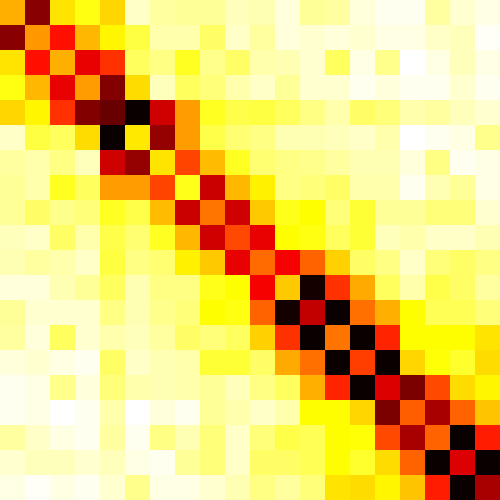
\includegraphics[width=8cm,height=8cm]{CTG_1_example.png}};

\pic[shift={(0,0,0)}] at (0,0,0) 
    {Box={
        name=conv1,
        caption= ,
        xlabel={{16, }},
        zlabel=,
        fill=\ConvColor,
        height=40,
        width=4,
        depth=40
        }
    };

\pic[shift={ (0,0,0) }] at (conv1-east) 
    {Box={
        name=bn1,
        caption= ,
        xlabel={{, }},
        fill=\PoolColor,
        opacity=0.5,
        height=40,
        width=2,
        depth=40
        }
    };

\pic[shift={(2,0,0)}] at (bn1-east) 
    {Box={
        name=anchor1_anchor,
        caption= ,
        xlabel={{, }},
        zlabel=,
        fill=\VoidColor,
        height=2,
        width=0,
        depth=2
        }
    };

\pic[shift={(2,0,0)}] at (bn1-east) 
    {Ball={
        name=anchor1,
        fill=\SumColor,
        opacity=1,
        radius=1.5,
        logo=
        }
    };

\draw [connection]  (bn1-east)    -- node {\midarrow} (anchor1-west);

\pic[shift={(2,0,0)}] at (anchor1-east) 
    {Box={
        name=resnext1_reduce,
        caption= ,
        xlabel={{, }},
        zlabel=,
        fill=\ConvColor,
        height=20,
        width=2,
        depth=20
        }
    };

\draw [connection]  (anchor1-east)    -- node {\midarrow} (resnext1_reduce-west);

\pic[shift={(4,0,3)}] at (resnext1_reduce-east) 
    {Box={
        name=resnext1_path1,
        caption= ,
        xlabel={{, }},
        zlabel=,
        fill=\ConvColor,
        height=20,
        width=2,
        depth=20
        }
    };

\draw [connection]  (resnext1_reduce-east)    -- node {\midarrow} (resnext1_path1-west);

\pic[shift={(4,0,9)}] at (resnext1_reduce-east) 
    {Box={
        name=resnext1_path2,
        caption= ,
        xlabel={{, }},
        zlabel=,
        fill=\ConvColor,
        height=20,
        width=2,
        depth=20
        }
    };

\draw [connection]  (resnext1_reduce-east)    -- node {\midarrow} (resnext1_path2-west);

\pic[shift={(4,0,-3)}] at (resnext1_reduce-east) 
    {Box={
        name=resnext1_path3,
        caption= ,
        xlabel={{, }},
        zlabel=,
        fill=\ConvColor,
        height=20,
        width=2,
        depth=20
        }
    };

\draw [connection]  (resnext1_reduce-east)    -- node {\midarrow} (resnext1_path3-west);

\pic[shift={(4,0,-9)}] at (resnext1_reduce-east) 
    {Box={
        name=resnext1_path4,
        caption= ,
        xlabel={{, }},
        zlabel=,
        fill=\ConvColor,
        height=20,
        width=2,
        depth=20
        }
    };

\draw [connection]  (resnext1_reduce-east)    -- node {\midarrow} (resnext1_path4-west);

\pic[shift={(9,0,0)}] at (resnext1_reduce-east) 
    {Ball={
        name=resnext1_concat,
        fill=\SumColor,
        opacity=1,
        radius=1.5,
        logo=$+$
        }
    };

\draw [connection]  (resnext1_path1-east)    -- node {\midarrow} (resnext1_concat-west);

\draw [connection]  (resnext1_path2-east)    -- node {\midarrow} (resnext1_concat-west);

\draw [connection]  (resnext1_path3-east)    -- node {\midarrow} (resnext1_concat-west);

\draw [connection]  (resnext1_path4-east)    -- node {\midarrow} (resnext1_concat-west);

\pic[shift={(1,0,0)}] at (resnext1_concat-east) 
    {Box={
        name=resnext1_restore,
        caption= ,
        xlabel={{, }},
        zlabel=,
        fill=\ConvColor,
        height=20,
        width=8,
        depth=20
        }
    };

\draw [connection]  (resnext1_concat-east)    -- node {\midarrow} (resnext1_restore-west);

\pic[shift={(1,0,0)}] at (resnext1_restore-east) 
    {Box={
        name=resnext1_sum_anchor,
        caption= ,
        xlabel={{, }},
        zlabel=,
        fill=\VoidColor,
        height=2,
        width=0,
        depth=2
        }
    };

\pic[shift={(1,0,0)}] at (resnext1_restore-east) 
    {Ball={
        name=resnext1_sum,
        fill=\SumColor,
        opacity=1,
        radius=1.5,
        logo=$+$
        }
    };

\draw [connection]  (resnext1_restore-east)    -- node {\midarrow} (resnext1_sum-west);

\pic[shift={(6,8,0)}] at (anchor1-east) 
    {Box={
        name=resnext1_shortcut,
        caption=Shortcut,
        xlabel={{, }},
        zlabel=,
        fill=\ConvColor,
        height=20,
        width=8,
        depth=20
        }
    };

\path (anchor1_anchor-southeast) -- (anchor1_anchor-northeast) coordinate[pos=20.5] (anchor1_anchor-top) ;
\path (resnext1_sum-south)  -- (resnext1_sum-north)  coordinate[pos=14] (resnext1_sum-top) ;
\draw [copyconnection]  (anchor1_anchor-northeast)  
-- node {\copymidarrow}(anchor1_anchor-top)
-- node {\copymidarrow}(resnext1_sum-top)
-- node {\copymidarrow} (resnext1_sum-north);

\pic[shift={ (1,0,0) }] at (resnext1_sum-east) 
    {Box={
        name=AvgPool,
        caption=,
        xlabel={{64, }},
        fill=\PoolColor,
        opacity=0.5,
        height=2,
        width=16,
        depth=2
        }
    };

\draw [connection]  (resnext1_sum-east)    -- node {\midarrow} (AvgPool-west);
\draw[dashed, thick, rounded corners, black, opacity=1]
    % Bottom-back corner of the box (x,y,z)
    (-1,-11,-10)
    % Forward in x (width)
    -- (15.5,-11,-10)
    % Up in y (height)
    -- (15.5,7.5,-10)
    % Back in x
    -- (-1,7.5,-10)
    % Down in y
    -- (-1,-11,-10)
    % Return in depth (z)
    -- cycle;
\node[align=center] at (14, -5, 0) {
    \textbf{ResNeXt blocks $\times$3}\\
    Cardinality: 4\\
    Filters: [32, 64, 64]\\
    Output size: [10$\times$10, 10$\times$10, 5$\times$5]\\
    Kernel size: 3$\times$3
};

\end{tikzpicture}
\end{document}
